\label{Organisation}

\section{Schedule}

As with any software project, planning is an important aspect. As is to be expected from a group without much prior experience in teamwork, the original schedule was overly optimistic. Other course deadlines and a failure to appreciate the time requirements of each stage resulted in a failure to meet our planned deadlines. 

\begin{figure}[!h]
    \begin{center}
        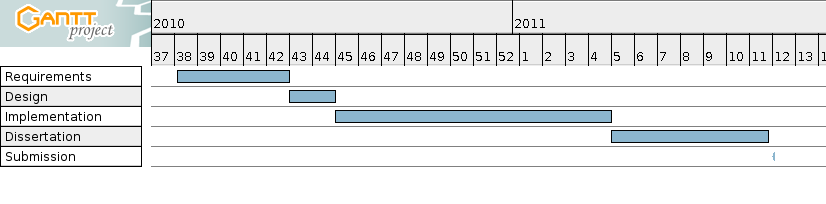
\includegraphics[width=7cm]{appendix/diagrams/GIMplan.png}
        \caption{Gantt chart of our planned schedule.}
        \label{lockingDia}
    \end{center}
\end{figure}

\begin{figure}[!h]
    \begin{center}
        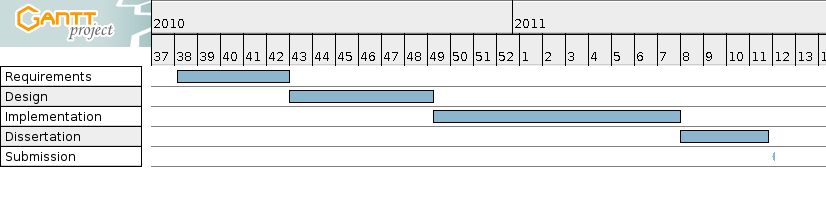
\includegraphics[width=7cm]{appendix/diagrams/GIMreal.png}
        \caption{Gantt chart of our actual schedule.}
        \label{lockingDia}
    \end{center}
\end{figure}

The process of designing the system took longer than was initially anticipated, which delayed the implementation process significantly. The implementation process for basic functionality went smoothly and was finished relatively quickly, however a significant amount of time was spent improving the interface and polishing the program.

\section{Management}


